\documentclass[a4paper, czech]{article}

\title{Úloha č.4: Bipolární tranzistor jako zesilovač}
\author{Karolína Andrea Šebestová}
\date{Datum měření: 28.3.2024}

\usepackage[czech]{babel}
\usepackage{indentfirst}
\usepackage{graphicx}
\usepackage{float}
\usepackage[margin=1.5cm]{geometry}
\usepackage{booktabs}
\usepackage{amsmath}
\usepackage{multirow}
\usepackage{colortbl}

\begin{document}

\maketitle

\section{Teoretický úvod}

Tranzistor se nejčastěji používá pro zesilování signálů. Pro jeho správnou funkci je třeba nastavit jeho pracovní bod. Ten je určen stejnosměrnými napětími a proudy na elektrodách tranzistoru, která jsou taková, aby emitorový přechod byl v propustném směru a kolektorový v závěrném a aby se tranzistor nacházel při nulovém střídavém vstupním napětí ve vhodné části svých charakteristik. Zapojení zesilovače se společným emitorem se základním nastavením pracovního bodu tranzistoru pomocí předřadného rezistoru $R_1$ je na Obr. 1. Je nutné poznamenat, že v praxi se používají složitější obvody pro nastavení pracovního bodu zejména kvůli zajištění jeho teplotní stability.

\begin{figure}[H]
    \centering
    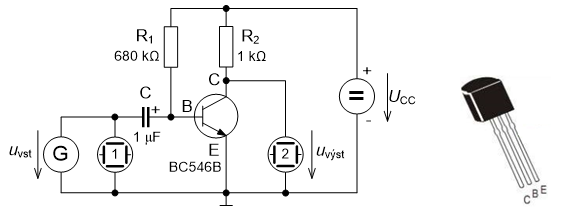
\includegraphics{zapojeni_SE.png}
    \caption{Zapojení se společným emitorem}
\end{figure}

\section{Seznam přístrojů}

\begin{enumerate}
    \item Osciloskop Agilent DSO-X 2002A
    \item Osciloskopická sonda HP 10074B
    \item Generátor Agilent 33521A
    \item Zdroj Agilent E3620A
    \item Multimetr Keysight 34461A
\end{enumerate}

\section{Úkoly měření}

Úkolem je změřit amplitudové kmitočtové a převodní charakteristiky bipolárního tranzistoru v zapojení se společným emitorem.

\begin{enumerate}
    \item Sestavte obvod podle Obr. 1. Přiveďte napájecí napětí $U_{CC} = 10 V$ a voltmetrem zkontrolujte, že napětí mezi kolektorem a emitorem $U_{CE}$ bez připojeného generátoru G je přibližně polovina napájecího napětí, tedy cca 5 V. Oba kanály osciloskopu nastavte na střídavou vazbu (stiskněte tlačítko s číslem kanálu 1 nebo 2, poté tlačítkem pod displejem Coupling vyberete AC). Signál do druhého kanálu osciloskopu přivádějte pomocí sondy. Černé krokodýlky koaxiálních kabelů a sondy připojujte k zemnímu, tedy ve schématu spodnímu, vodiči. Aby osciloskop ukazoval na kanále se sondou správné napěťové hodnoty, zmáčkněte tlačítko čísla kanálu 2, poté pod displejem Probe a v položce Probe nastavte pomocí kolečka s prosvětlenu šipkou 10.0:1. Vzhledem k malým hodnotám vstupního napětí je vhodné osciloskop synchronizovat na výstupní napětí, tedy na kanál 2. To provedete stiskem tlačítka Trigger a na displeji zvolíte Source 2. Knoflíkem Trigger pak nastavte úroveň synchronizace zhruba doprostřed průběhu na kanálu 2.   
    \item Změřte závislost zesílení zesilovače $A_{UdB} = 20 log ( U_{vyst} / U_{vst} )$ na frekvenci. Vstupní napětí nastavte přibližně 40 mV špička-špička (na generátoru nutno nastavit polovinu, tedy 20 mVpp), sinusový průběh a frekvenci měňte od 100 Hz do 5 MHz v přibližně 20 hodnotách. Pro aktivaci výstupu generátoru je třeba stisknout tlačítko Channel a poté tlačítkem pod displejem nastavit Output on. Frekvenční krok volte přibližně logaritmicky a zjemněte jej při větších změnách výstupního napětí, aby bylo možné v grafu dobře spojit měřené body hladkou čarou. Vstupní i výstupní napětí ($U_{vst}, U_{vyst}$) měřte na osciloskopu pomocí funkce tlačítka Meas, tlačítkem Type pod displejem zvolte Peak-Peak a tlačítkem Source vyberte měřený kanál. Volbu potvrďte pomocí Add Measurement.
    \item Změřenou závislost zesílení na frekvenci vyneste do grafu. Na vodorovné (frekvenční) ose použijte logaritmické měřítko, na svislé ose (zesílení $A_{UdB}$ v dB) použijte měřítko lineární. Odečtěte maximální hodnotu zesílení a kmitočet, na kterém toto maximum nastává. Zjistěte mezní kmitočet, kde klesne zesílení o 3 dB oproti maximálnímu zesílení.
    \item Změřte převodní charakteristiku zesilovače, tedy závislost velikosti výstupního napětí Uvýst na vstupním napětí $U_{vst}$. Použijte opět zapojení podle Obr. 1, na generátoru nastavte sinusový průběh, kmitočet 1 kHz a vstupní napětí $U_{vst}$ měňte od 10 mV do 100 mV špička-špička (na generátoru 5 mVpp až 50 mVpp). Změřte přibližně 20 hodnot. Na osciloskopu odečítejte mezivrcholové hodnoty vstupního a výstupního napětí opět pomocí funkce Meas. Časové průběhy vstupního a výstupního napětí pro $U_{vst}$ 10 mV a 100 mV špička-špička vložte (jako čitelnou fotku obrazovky nebo uložením na USB) či obkreslete do protokolu. Graficky znázorněte závislost výstupního napětí na vstupním s lineárními měřítky na obou osách. Zhodnoťte, ve které oblasti lze charakteristiku považovat za lineární. Také popište na osciloskopu pozorované změny v časovém průběhu výstupního napětí při zvyšování vstupního napětí.
\end{enumerate}

\section{Naměřené a vypočtené hodnoty}

V této sekci se nachází dvě tabulky.
Naměřené i vypočtené hodnoty amplitudové kmitočtové charakteristiky jsme vynesli do jedné společné tabulky.
Ve druhé tabulce se nachází naměřené hodnoty přenosové charakteristiky.

Dále se zde nachází i časové průběhy vstupního a výstupního napětí pro $U_{vst}$ 10 mV špička-špička a 100 mV špička-špička uložené z osciloskopu.

Slovní popis symbolů veličin:
$f$ - frekvence;
$U_{vst}$ - vstupní napětí špička-špička;
$U_{vyst}$ - výstupní napětí špička-špička;
$A_{UdB}$ - zesílení zesilovače v dB

\begin{table}[H]
    \centering
    \begin{tabular}{ccccc}
        \multicolumn{5}{c}{$U_{CC} = 10V$} \\
        \toprule
        $*$  & $f\ (Hz)$    & $U_{vst}\ (mVpp)$ & $U_{vyst}\ (Vpp)$ & $A_{UdB}\ (dB)$ \\
        \midrule
        1  & 100       & 41        & 3,9       & 39,57     \\
        2  & 250       & 41        & 4,7       & 41,19     \\
        3  & 500       & 41        & 5         & 41,72     \\
        4  & 750       & 41        & 5,1       & 41,90     \\
        5  & 1 000     & 41        & 5,1       & 41,90     \\
        6  & 2 500     & 41        & 5,1       & 41,90     \\
        7  & 5 000     & 41        & 5,1       & 41,90     \\
        8  & 7 500     & 41        & 5,1       & 41,90     \\
        9  & 10 000    & 41        & 5,1       & 41,90     \\
        10 & 25 000    & 41        & 5,1       & 41,90     \\
        11 & 50 000    & 41        & 4,9       & 41,55     \\
        12 & 75 000    & 41        & 4,8       & 41,37     \\
        13 & 100 000   & 41        & 4,7       & 41,19     \\
        14 & 250 000   & 41        & 4,5       & 40,81     \\
        15 & 500 000   & 40        & 4,3       & 40,63     \\
        16 & 750 000   & 39        & 4,1       & 40,43     \\
        17 & 1 000 000 & 38        & 3,9       & 40,23     \\
        18 & 2 500 000 & 33        & 2,5       & 37,59     \\
        19 & 5 000 000 & 33        & 1,2       & 31,21     \\
        \bottomrule
    \end{tabular}
    \caption{Naměŕené a vypočtené hodnoty amplitudové kmitočtové charakteristiky}
\end{table}

\begin{table}[H]
    \centering
    \begin{tabular}{ccc}
        \multicolumn{3}{c}{$f = 1kHz$} \\
        \toprule
        $*$  & $U_{vst}\ (mVpp)$ & $U_{vyst}\ (Vpp)$ \\
        \midrule
        1  & 11        & 1,4       \\
        2  & 16        & 2,1       \\
        3  & 21        & 2,7       \\
        4  & 27        & 3,3       \\
        5  & 31        & 3,9       \\
        6  & 36        & 4,4       \\
        7  & 41        & 5,1       \\
        8  & 46        & 5,5       \\
        9  & 51        & 6,1       \\
        10 & 55        & 6,6       \\
        11 & 60        & 7         \\
        12 & 65        & 7,5       \\
        13 & 70        & 7,9       \\
        14 & 76        & 8,4       \\
        15 & 80        & 8,7       \\
        16 & 85        & 9         \\
        17 & 90        & 9,1       \\
        18 & 95        & 9,2       \\
        19 & 100       & 9,3       \\
        \bottomrule
    \end{tabular}
    \caption{Naměřené hodnoty přenosové charakteristiky}
\end{table}

Na následujícím naměřeném průběhu je patrné, že při nízkém vstupním napětí $U_{vst}$ že dochází k velkému zesílení a zároveň nedochází k velkému zkreslení výstupního signálu.

\begin{figure}[H]
    \centering
    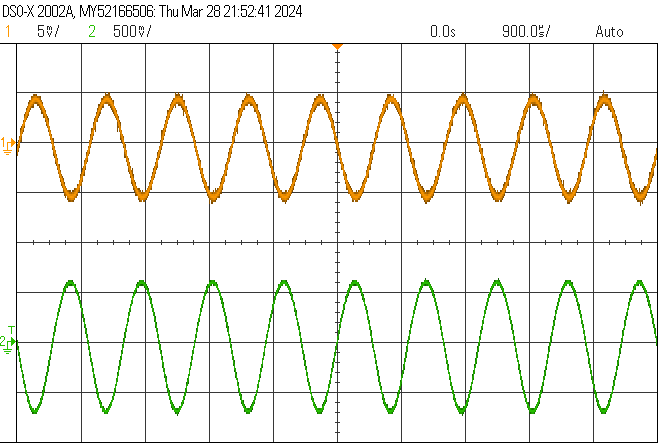
\includegraphics{prubeh_10mVpp.png}
    \caption{Časový průběh vstupního a výstupního napětí pro $U_{vst} =  10 mV$}
\end{figure}

Na průběhu s vyšším vstupním napětím $U_{vst}$ je však zřejmé, že dochází ke značnému zkreslení. Je patrné, že dochází k "ořezu" ve vrchní části průběhu.

\begin{figure}[H]
    \centering
    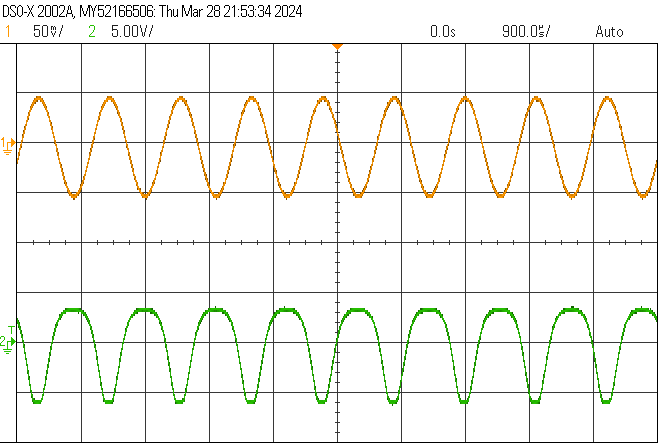
\includegraphics{prubeh_100mVpp.png}
    \caption{Časový průběh vstupního a výstupního napětí pro $U_{vst} =  100 mV$}
\end{figure}

\section{Příklady výpočtu}

Závislost zesílení zesilovače $A_{UdB}$ na frekvenci $f$ byla vypočtena podle následujícího vztahu:

$$A_{UdB}=20 \cdot \log\left(\frac{U_{vyst}}{U_{vst}}\right)$$

Uvedeme si konkrétní příklad výpočtu pro první řádek tabulky naměřených hodnot:

$${A_{UdB}}_1 = 20 \cdot \log\left(\frac{U_{vyst}}{U_{vst}}\right) = 20 \cdot \log\left(\frac{3,9 V}{41 \cdot 10^{-3}V}\right) \approx \underline{\underline{39,57 dB}}$$

\section{Grafy}

Naměřené hodnoty zesílení $A_{UdB}$ byly vyneseny do grafu jako funkce frekcence $f$, která je zobrazena v logaritmickém měřítku. Výsledný graf tedy tvoří amplitudovou kmitočtovou charakteristiku.
Maximální hondota zesílení je $A_{UdB} = 41,90dB$ a toto maximum nastává na kmitočtovém intervalu $750 Hz$ až $25 kHz$.
Mezní kmitočet, kde zesílení klesne o $3 dB$ rovné hodnotě $38,9 dB$ oproti maximálnímu zesílení byl odečten z grafu a přibližně se rovná hodnotě $1,6 MHz$.

\begin{figure}[H]
    \centering
    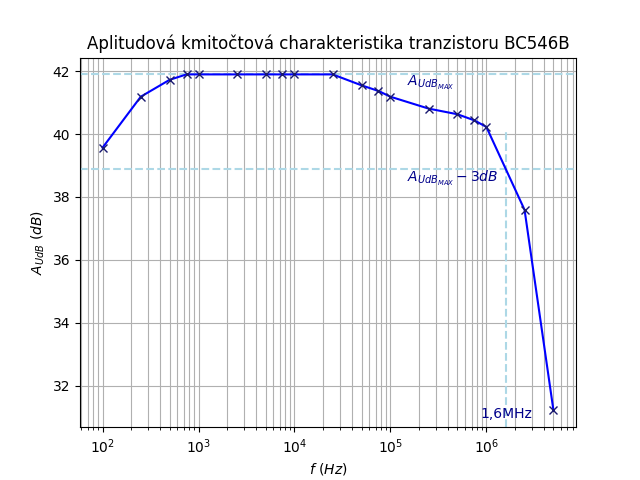
\includegraphics{akch.png}
    \caption{Naměřená amplitudová kmitočtová charakteristika vynesena do grafu}
\end{figure}

Převodní charakteristika zesilovače je zobrazena jako závislost naměřených mezivrcholových hodnot výstupního napětí $U_{vyst}$ na vstupním napětí $U_{vst}$.
Ve vyhotoveném grafu je oblast, kterou je možné považovat za lineární ilustračně proložena lineární funkcí.
V posledních čtyřech naměŕených bodech dochází k velkému "ohybu" charakteristiky, proto nejsou zahrnuty do lineární části.

\begin{figure}[H]
    \centering
    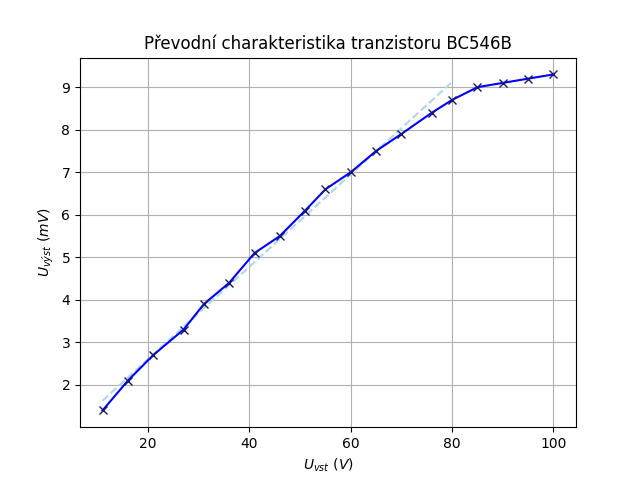
\includegraphics{pch.png}
    \caption{Naměřená přenosová charakteristika vynesena do grafu}
\end{figure}

\section{Závěr}

Jako první jsme měřili závislost zesílení zesilovače $A_{UdB}$ na frekvenci $f$, neboli amplitudovou kmitočtou charakteristiku.
Naměřené hodnoty byly vyneseny do grafu, kde pro frekvenci bylo použito logaritmické měřítko
V této charakteristice byly použity horizontální přímky pro odečtení maximální hodnoty zesílení $A_{UdB_{MAX}}$ a poklesu maximálního zesílení o 3dB.
Další vertikální křivka byla použita pro odečtení mezního kmitočtu, kde k tomuto poklesu došlo.
Zjistili jsme, že k maximálnímu zesílení dochází na intervalu frekvenčních hodnot od 750Hz až po 25kHz.
Mezní kmitočet, kde dochází k poklesu zesílení o 3dB oproti maximální hodnotě je přibližně roven 1,6MHz.

Dále jsme měřili převodní charakteristiku zesilovače, neboli závislost velikosti výstupního napětí na vstupním napětí při konstantním kmitočtu.
Naměřené hodnoty byly vyneseny do grafu s lineárními osami.
Pro zhodnocení, ve které oblasti lze charakteristiku považovat za lineární jsme charakteristiku proloži pomocnou lineání funkcí.
Pomocí ní je zřejmé, že charakteristika je přibližně lineární v rozsahu hodnot vstupního napětí 11mVpp až 80mVpp.
Při vyšších hodnotách vstupního napětí už dochází k přiliš velkému "ohybu" charakteristiky, proto tyto hodnoty nemůžeme považovat ani za přibližně lineání.

Během měření jsme pozorovali také změny v časovém průběhu výstupního napětí.
Tyto změny jsou patrné v obrázcích 2 a 3.
Je vidět, že při nižších hodnotách vstupního napětí dochází k zesílení bez žádného výrazného zkreslení.
Při vysokých hodnotách vstupního napětí však už dochází k výrazném uzkreslení výstupního signálu a ten je navíc i patrně "ořezán" ve vrchní části.

\end{document}